% Aumento de SNR x potência (Resultados), separado de hardware.tex em 2026-11-09 para fechar o
%   capítulo, como a última pergunta do roteiro da autora.
% =====================================================================
\section{\texorpdfstring{\textcolor{red}{Aumento de SNR e potência}}{Aumento de SNR e potência}}\label{subsec:resultados-compromisso}
% =====================================================================
% FONTE: analise_potencia_qualidade.py (quadrantes_cond_g1/_g3 e _data.csv,
%   tabela_escolha_condicao, escolha_cond). Qualidade: grade_inteira.py (mesmos dados das barras
%   e curvas). TDLA30-10 usa a simulação da TDLA30-5. Pior caso A-H = pior caso E-H em todos os
%   pontos dos grupos 1 e 3 (conferido no script). G1, <26,12>, TDLA30-5 e -10: 0,104 dB.

\textcolor{red}{As Figuras~\ref{fig:quadrantes-g1} e \ref{fig:quadrantes-g3} juntam o aumento de SNR e a potência dinâmica nos grupos 1 e 3. Cada ponto é um formato numa condição de teste. No eixo x, está o pior aumento de SNR entre as configurações do grupo com o IoTh do gráfico, naquela condição: 10~dB (A a D) à esquerda e 20~dB (E a H) à direita. No gráfico da direita, o pior caso é o mesmo de todo o grupo (A a H). No eixo y, está a potência dinâmica do formato na arquitetura da condição, e a linha horizontal marca a potência estática.}


\textcolor{red}{Só os grupos 1 e 3 aparecem, porque eles usam o circuito $16 \times 16$. No grupo 2 ($32 \times 32$), só a versão sem otimização foi implementada, e ela não atende nenhum limite. A potência foi medida só com matrizes do grupo 1 (Seção~\ref{subsec:hw-matrizes}), e isso é uma limitação para o grupo 3. Mas os dados de entrada parecem mudar pouco a potência: na versão sem otimização do $\langle 18,8\rangle$, medida com as matrizes de cada uma das 5 condições de teste, a potência dinâmica ficou entre 0,031 e 0,032~W.}


\begin{figure}[!ht]
\caption{\textcolor{red}{Aumento de SNR e potência dinâmica de cada formato nas condições de teste, grupo 1.}}
\label{fig:quadrantes-g1}
\vspace{4pt} % a classe zera o espaço entre a caption e a figura
\centering
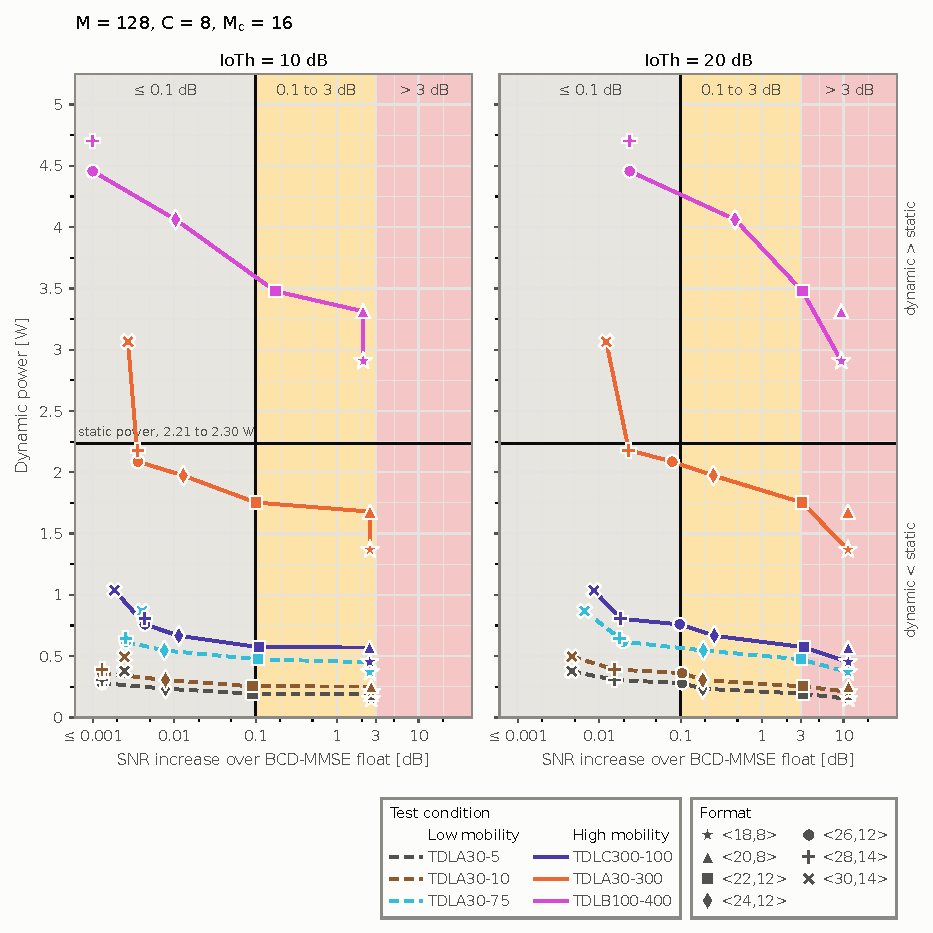
\includegraphics[width=\textwidth]{Images/RESULTADOS/quadrantes_cond_g1.pdf}
\vspace{4pt}
\legend{\textcolor{red}{Fonte: a autora. Linha tracejada: baixa mobilidade; cheia: alta mobilidade. As linhas ligam os formatos que nenhum outro supera ao mesmo tempo em aumento de SNR e em potência.}}
\end{figure}

\begin{figure}[!ht]
\caption{\textcolor{red}{Aumento de SNR e potência dinâmica de cada formato nas condições de teste, grupo 3.}}
\label{fig:quadrantes-g3}
\vspace{4pt} % a classe zera o espaço entre a caption e a figura
\centering
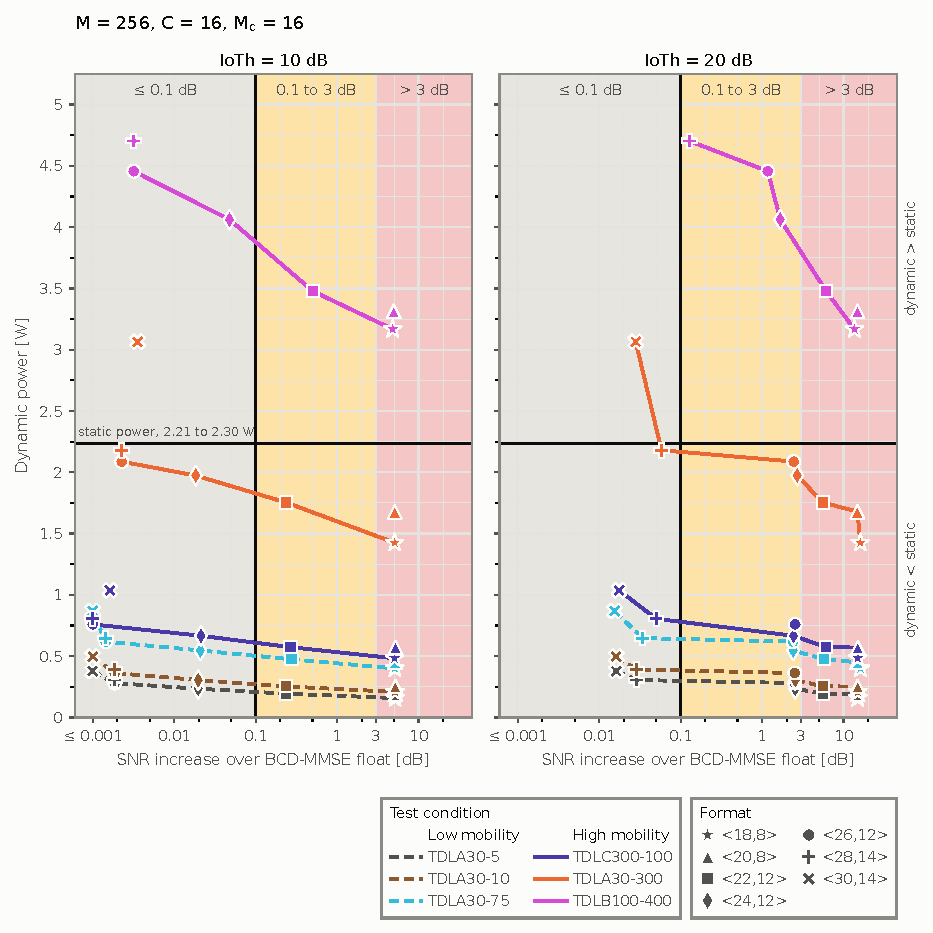
\includegraphics[width=\textwidth]{Images/RESULTADOS/quadrantes_cond_g3.pdf}
\vspace{4pt}
\legend{\textcolor{red}{Fonte: a autora. Linha tracejada: baixa mobilidade; cheia: alta mobilidade. As linhas ligam os formatos que nenhum outro supera ao mesmo tempo em aumento de SNR e em potência.}}
\end{figure}

\textcolor{red}{Como a potência muda mais com a arquitetura do que com o formato (Seção~\ref{subsec:resultados-potencia}), cada condição forma uma faixa de altura própria nas figuras. A Tabela~\ref{tab:escolha-condicao} mostra o formato escolhido em cada condição de teste: o menor que cabe na arquitetura e fica dentro do limite.}


\textcolor{red}{No grupo 1, com IoTh de 20~dB, o limite de 3~dB fica no $\langle 24,12\rangle$ em quase todas as condições. Na TDLA30-75, o $\langle 22,12\rangle$ já basta, com 2,97~dB. Para 0,1~dB, todas as condições usam o $\langle 26,12\rangle$. Na TDLA30-5 e na TDLA30-10, ele fica em 0,104~dB, que arredonda para 0,10~dB. Passar de 3~dB para 0,1~dB aumenta a potência dinâmica de 6\% (TDLA30-300) a 30\% (TDLA30-75).}


\textcolor{red}{Na TDLB100-400, o $\langle 24,12\rangle$ fica 0,47~dB acima do BCD-MMSE em ponto flutuante. Esse aumento pede que cada UE transmita 11\% mais energia por símbolo (Seção~\ref{subsec:aumento-snr}). O $\langle 26,12\rangle$ tira essa diferença com 0,39~W a mais de potência dinâmica no FPGA.}


\textcolor{red}{No grupo 3, com IoTh de 20~dB, o limite de 3~dB fica no $\langle 24,12\rangle$ em todas as condições. O de 0,1~dB fica no $\langle 28,14\rangle$, com 10 a 30\% mais potência dinâmica. Na TDLB100-400, nenhum formato que cabe no FPGA atende 0,1~dB. O $\langle 28,14\rangle$ fica em 0,13~dB, e o $\langle 30,14\rangle$ não cabe.}


\textcolor{red}{Com IoTh de 10~dB, os formatos ficam menores e só mudam entre as condições no grupo 1, para 0,1~dB: na TDLA30-5, na TDLA30-10 e na TDLA30-300, basta o $\langle 22,12\rangle$.}


\begin{table}[htbp]
\caption{\textcolor{red}{Formato escolhido em cada condição de teste, com o pior aumento de SNR, em dB, e a potência dinâmica, em W.}}
\label{tab:escolha-condicao}
\vspace{4pt} % a classe zera o espaço entre a caption e a tabela
\centering
\scriptsize
\color{red}
\renewcommand{\arraystretch}{1.2}
\setlength{\tabcolsep}{2.2pt}
\begin{tabular}{lcccccccccccc}
\toprule
 & \multicolumn{6}{c}{\textbf{IoTh of 10~dB (A to D)}} & \multicolumn{6}{c}{\textbf{IoTh of 20~dB (E to H)}} \\
\cmidrule(lr){2-7}\cmidrule(lr){8-13}
 & \multicolumn{3}{c}{\textbf{Up to 3 dB}} & \multicolumn{3}{c}{\textbf{Up to 0.1 dB}} & \multicolumn{3}{c}{\textbf{Up to 3 dB}} & \multicolumn{3}{c}{\textbf{Up to 0.1 dB}} \\
\cmidrule(lr){2-4}\cmidrule(lr){5-7}\cmidrule(lr){8-10}\cmidrule(lr){11-13}
\textbf{Test condition} & \textbf{Format} & \textbf{dB} & \textbf{W} & \textbf{Format} & \textbf{dB} & \textbf{W} & \textbf{Format} & \textbf{dB} & \textbf{W} & \textbf{Format} & \textbf{dB} & \textbf{W} \\
\midrule
\multicolumn{13}{l}{\textbf{Group 1 ($M$ = 128, $C$ = 8)}} \\
\multicolumn{13}{l}{Low mobility} \\
\quad TDLA30-5 & $\langle 18,8\rangle$ & 2.62 & 0.15 & $\langle 22,12\rangle$ & 0.09 & 0.19 & $\langle 24,12\rangle$ & 0.19 & 0.23 & $\langle 26,12\rangle$ & 0.10 & 0.28 \\
\quad TDLA30-10 & $\langle 18,8\rangle$ & 2.62 & 0.21 & $\langle 22,12\rangle$ & 0.09 & 0.25 & $\langle 24,12\rangle$ & 0.19 & 0.30 & $\langle 26,12\rangle$ & 0.10 & 0.36 \\
\quad TDLA30-75 & $\langle 18,8\rangle$ & 2.52 & 0.37 & $\langle 24,12\rangle$ & 0.01 & 0.55 & $\langle 22,12\rangle$ & 2.97 & 0.47 & $\langle 26,12\rangle$ & 0.02 & 0.62 \\
\multicolumn{13}{l}{High mobility} \\
\quad TDLC300-100 & $\langle 18,8\rangle$ & 2.51 & 0.45 & $\langle 24,12\rangle$ & 0.01 & 0.67 & $\langle 24,12\rangle$ & 0.26 & 0.67 & $\langle 26,12\rangle$ & 0.10 & 0.76 \\
\quad TDLA30-300 & $\langle 18,8\rangle$ & 2.53 & 1.37 & $\langle 22,12\rangle$ & 0.10 & 1.75 & $\langle 24,12\rangle$ & 0.25 & 1.97 & $\langle 26,12\rangle$ & 0.08 & 2.09 \\
\quad TDLB100-400 & $\langle 18,8\rangle$ & 2.09 & 2.91 & $\langle 24,12\rangle$ & 0.01 & 4.06 & $\langle 24,12\rangle$ & 0.47 & 4.06 & $\langle 26,12\rangle$ & 0.02 & 4.46 \\
\midrule
\multicolumn{13}{l}{\textbf{Group 3 ($M$ = 256, $C$ = 16)}} \\
\multicolumn{13}{l}{Low mobility} \\
\quad TDLA30-5 & $\langle 22,12\rangle$ & 0.23 & 0.19 & $\langle 24,12\rangle$ & 0.02 & 0.23 & $\langle 24,12\rangle$ & 2.55 & 0.23 & $\langle 28,14\rangle$ & 0.03 & 0.30 \\
\quad TDLA30-10 & $\langle 22,12\rangle$ & 0.23 & 0.25 & $\langle 24,12\rangle$ & 0.02 & 0.30 & $\langle 24,12\rangle$ & 2.55 & 0.30 & $\langle 28,14\rangle$ & 0.03 & 0.39 \\
\quad TDLA30-75 & $\langle 22,12\rangle$ & 0.28 & 0.47 & $\langle 24,12\rangle$ & 0.02 & 0.55 & $\langle 24,12\rangle$ & 2.40 & 0.55 & $\langle 28,14\rangle$ & 0.03 & 0.65 \\
\multicolumn{13}{l}{High mobility} \\
\quad TDLC300-100 & $\langle 22,12\rangle$ & 0.27 & 0.57 & $\langle 24,12\rangle$ & 0.02 & 0.67 & $\langle 24,12\rangle$ & 2.44 & 0.67 & $\langle 28,14\rangle$ & 0.05 & 0.81 \\
\quad TDLA30-300 & $\langle 22,12\rangle$ & 0.24 & 1.75 & $\langle 24,12\rangle$ & 0.02 & 1.97 & $\langle 24,12\rangle$ & 2.70 & 1.97 & $\langle 28,14\rangle$ & 0.06 & 2.18 \\
\quad TDLB100-400 & $\langle 22,12\rangle$ & 0.50 & 3.48 & $\langle 24,12\rangle$ & 0.05 & 4.06 & $\langle 24,12\rangle$ & 1.67 & 4.06 & -- & -- & -- \\
\bottomrule
\end{tabular}
\vspace{4pt}
\legend{\textcolor{red}{Fonte: a autora. Menor formato que cabe na arquitetura da condição de teste e cujo pior aumento de SNR, entre as configurações com aquele IoTh, fica até o limite. Modo \texttt{AP\_RND\_ZERO}/\texttt{AP\_WRAP}. --: nenhum formato que cabe no FPGA atende o limite.}}
\end{table}
